\documentclass[conference]{IEEEtran}
\usepackage{amsmath,amssymb}
\usepackage{graphicx}
\usepackage{booktabs}
\usepackage{siunitx}
\usepackage{cite}
\usepackage[hidelinks]{hyperref}
\graphicspath{{../results/}}
\sisetup{group-digits=false}
\setlength{\textfloatsep}{8pt plus 2pt minus 2pt}

\begin{document}
\title{Per-Step Cost of a Python EMT Solver\\and Requirements for Real-Time Execution}
\author{\IEEEauthorblockN{Haoran Liu}
\IEEEauthorblockA{CloudDRTS preparation, Phase 4}}
\maketitle

\begin{abstract}
The partitioned test circuit of Phase 3 is timed step by step in four implementations of the same computation, from the general nodal solver to a compiled loop. The general solver needs \SI{15.2}{\micro\second} per step (median), the compiled loop \SI{12}{ns}; most of the difference is interpreter and function-call overhead. Even the fastest interpreted version shows occasional steps far longer than its median, which rules out interpreted code for hard real-time execution. The note ends with questions to be settled at the start of the project.
\end{abstract}
\begin{IEEEkeywords}
Real-time simulation, electromagnetic transients, profiling, latency.
\end{IEEEkeywords}

\section{Introduction}
A real-time simulator must finish every step within the step length, not only on average~\cite{faruque}. This note measures what limits the Python solver of Phase~2 in this respect, as a basis for the move to compiled and FPGA implementations~\cite{chen,hls}.

\section{Set-Up}
The Phase~3 circuit is run as two solvers coupled by the Bergeron line (\SI{60}{Hz} source, $\Delta t=\SI{5}{\micro\second}$, 10\,000 steps including both switching events). Every step is timed with \texttt{time.perf\_counter\_ns}, and each measurement is repeated five times. Four implementations are compared; they produce the same waveform within \SI{1.4e-13}{V}:
\begin{itemize}
\item \emph{generic}: the general \texttt{Circuit} class for each subsystem, with \texttt{numpy.linalg.solve} in every step;
\item \emph{cached}: the same objects, with the inverse matrix of each switch state computed once;
\item \emph{scalar}: the two one-node subsystems written out with Python floating-point numbers;
\item \emph{compiled}: the scalar loop compiled with Numba, for which only the mean time per step can be measured.
\end{itemize}
The measurements were made on an x86-64 machine with Python 3.12 and NumPy 2.3; the tail values vary between runs.

\section{Results}
\begin{table}[!b]
\caption{Time per Step (\si{\micro\second}) and Share of Steps Exceeding the Step Length}
\label{tab:time}
\centering\footnotesize\setlength{\tabcolsep}{3.5pt}
\begin{tabular}{@{}lccccc@{}}
\toprule
Implementation & Median & 99th pct. & Max. & $>\SI{5}{\micro\second}$ & $>\SI{50}{\micro\second}$\\
\midrule
generic & 15.2 & 24.2 & 181 & \SI{100}{\percent} & \SI{0.05}{\percent}\\
cached & 7.9 & 11.1 & 584 & \SI{100}{\percent} & \SI{0.03}{\percent}\\
scalar & 0.28 & 0.36 & 26 & \SI{0.02}{\percent} & 0\\
compiled & 0.012 (mean) & -- & -- & -- & --\\
\bottomrule
\end{tabular}
\end{table}
\begin{figure}[!t]
\centering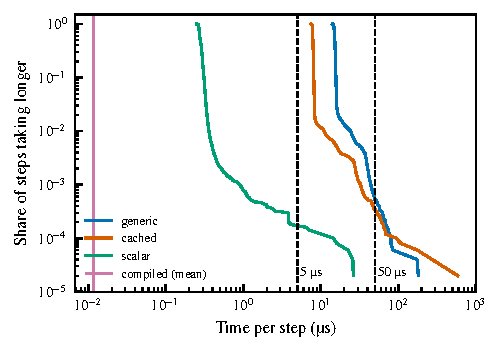
\includegraphics[width=\columnwidth]{phase4_timing.pdf}
\caption{Share of steps taking longer than a given time. Dashed lines: step lengths of 5 and \SI{50}{\micro\second}.}
\label{fig:time}
\end{figure}
Table~\ref{tab:time} and Fig.~\ref{fig:time} summarize the measurements.

One step of this circuit requires a few tens of floating-point operations, which the compiled loop executes in \SI{12}{ns}. The generic solver takes more than 1000 times longer, so the cost is dominated by overhead rather than by arithmetic. According to the profile, \texttt{numpy.linalg.solve} accounts for \SI{55}{\percent} of the run time, mostly argument checking and dispatch for a $1\times1$ system, and the Python code of the step function for most of the remainder.

Reusing one factorization per switch state halves the median, but every step still exceeds a \SI{5}{\micro\second} budget. Writing the update out with scalars brings the median to \SI{0.28}{\micro\second}.

For real-time operation, however, the distribution tail matters more than the median. Even the scalar loop has steps of up to \SI{26}{\micro\second}, and single steps of the other versions take hundreds of microseconds, as is typical of garbage collection and operating-system scheduling. A fixed-step real-time simulator requires a bound on the worst case, which interpreted code on a general-purpose operating system cannot provide. Compiled code on isolated processor cores, or an FPGA with a fixed schedule~\cite{chen}, is required.

For larger subsystems the arithmetic per step grows with the network size (sparse solution and history updates). With a fixed set of switch states the factorizations can be prepared in advance, as in the cached version, leaving forward and backward substitution in each step.

\section{Questions for the First Week}
\begin{enumerate}
\item \emph{Step length and budget}: which step is targeted for the prototype (\SI{50}{\micro\second} for the Kundur system, a few microseconds for converter models), and how is the budget divided between solution, interface exchange and input/output on the laboratory platforms?
\item \emph{Latency budget of a cut}: a cut at a line is exact while the latency stays below the travel time minus one step (about \SI{0.39}{ms} for a \SI{110}{km} tie section). Which lines in the target systems are long enough for the expected network latency, and how should a network be cut where no such line exists?
\item \emph{Message content}: should each message carry a time stamp and sequence number so that late or lost values are detected, and should a late value be held, extrapolated, or stop the simulation?
\item \emph{Equivalents}: is a frequency-dependent network equivalent obtained by vector fitting~\cite{vf}, together with aggregated machines, the intended representation of remote areas, and how is passivity of the fitted model ensured?
\item \emph{Accuracy metrics}: which errors matter to the industry partners: waveform RMS error, protection quantities such as peak fault current and detection time, or electromechanical quantities such as inter-area damping?
\item \emph{FPGA arithmetic}: which word length and scaling are needed for history terms and node voltages during faults, and is the FPGA solver generated per network with high-level synthesis~\cite{hls} or a programmable solver engine as in~\cite{chen}?
\item \emph{Reference system}: should the prototype use the network of Kundur's Example 12.6, whose data are complete, or that of Klein, Rogers and Kundur?
\end{enumerate}

\begin{thebibliography}{1}
\bibitem{faruque} M.~O. Faruque \emph{et al.}, ``Real-time simulation technologies for power systems design, testing, and analysis,'' \emph{IEEE Power Energy Technol. Syst. J.}, vol.~2, no.~2, pp.~63--73, 2015.
\bibitem{chen} Y.~Chen and V.~Dinavahi, ``FPGA-based real-time EMTP,'' \emph{IEEE Trans. Power Del.}, vol.~24, no.~2, pp.~892--902, Apr. 2009.
\bibitem{hls} AMD, \emph{Vitis High-Level Synthesis User Guide} (UG1399).
\bibitem{vf} B.~Gustavsen and A.~Semlyen, ``Rational approximation of frequency domain responses by vector fitting,'' \emph{IEEE Trans. Power Del.}, vol.~14, no.~3, pp.~1052--1061, Jul. 1999.
\end{thebibliography}
\end{document}
